\chapter{Reference Board}
\label{chap:reference}

A custom printed circuit board (PCB) was created for this thesis. The board is planned to be used as development platform to showcase possible IoT applications that can be benefit from using an ultra-low power accelerometer.

\section{Board specification}

The reference board is comprised of a nRF51 system-on-chip (SoC), an accelerometer, a voltage regulator, four LEDs and two tactile switches. Which accelerometer that is going to be used for the reference board will be determined after an analysis of the accelerometers presented in the overview in Chapter \ref{chap:overview}. This analysis is presented in Chapter \ref{chap:analysis}.

%A schematic of the demo board can be viewed in Appendix \ref{chap:appendix_a}.

\subsection{nRF51}

The nRF51 is a Cortex-M0+ based System-on-Chip (SoC) from Nordic Semiconductor. The company is world leading in creating Bluetooth Low Energy solutions. This SoC was chosen mainly because of its advanced power saving features, of which some of them will be presented in the following sections. 

\subsubsection{PPI}

The nRF51 has something the company calls Programmable Peripheral Interconnect (PPI), which essentially is the same as an event system (See Chapter \ref{chap:theory}). The PPI enables different peripherals in the device to interact autonomously with each other by using tasks and events \cite[~p.26]{nrf51}. The PPI can automatically trigger a task in one peripheral as a result of an event occurring in another. 

\subsubsection{GPIOTE}

The GPIO task and event system (GPIOTE) is a peripheral module in the nRF51 that is designed specifically for autonomous operation. The GPIOTE module is meant to work in conjunction with the PPI system \cite[~p.35]{nrf51}. A typical setup is to configure a pin with GPIOTE to listen for an external interrupts. When an external interrupt is detected on this pin, the PPI system can notify another peripheral about this event, which in turn can trigger another operation.

\subsubsection{EasyDMA}

The DMA (called EasyDMA) function in the nRF51 is able to move data to and from RAM and autonomously between peripherals \cite[~p.34]{nrf51}. EasyDMA can be configured to work in conjunction with the PPI system for execution of fully autonomous operations. For instance, an interrupt from an external device (i.e. accelerometer) can trigger the SPI module to initiate a DMA block transfer to memory, or to the radio. This essentially creates a sensor data acquisition system that is able to collect accelerometer data and send it over radio without using the CPU. It is however worth mentioning that the EasyDMA interface of the nRF51 does not support I2C.

\subsubsection{Bluetooth low energy}

Bluetooth Low Energy (BLE) is wireless communication protocol designed by the Bluetooth Special Interest Group (Bluetooth SIG), which Nordic Semiconductor is a part of. The protocol is aimed at healthcare, fitness and beacon applications. It is designed to have ultra-low peak, average and idle mode power consumption. This enables devices that uses BLE to run for years on a standard coin-cell battery \cite{ble}. BLE has become a big part of IoT applications that are available today, and is considered to be an important protocol for future devices as well. Another benefit with BLE, is that most of todays smart phones support the protocol and are therefore able to talk to other BLE devices. Low-power and smart phone connectivity was the main reason that BLE was chosen for this reference board. 

\section{Data acquisition scheme}

The reference board was designed with ultra-low power operation in mind. This section presents the planned data acquisition scheme for the reference board. The essence of the scheme is to only utilize low power peripherals to acquire data in such a way that the entire operation can be accomplished without using any CPU intervention  

The theoretical configuration uses EasyDMA, PPI, GPIOTE, SPI and the radio of the nRF51, as viewed with red boxes in Figure \ref{fig:nrf51}. The Cortex-M0+ CPU core should only be used for configuration of the system, and will be sleeping during data collection. The accelerometer will act as the system power switch by utilizing a low power motion activated wake-up mode. When a motion is detected above a predefined threshold, the accelerometer will signal an interrupt to nRF51. The PPI will be configured to listen to for this interrupt and to trigger a SPI block transfer when it is detected. As data is being transferred to the SPI module, the EasyDMA can shuffle data into RAM. This data can further be broadcasted by the radio. This entire operation should be possible to do without any CPU intervention at all.

\begin{figure}[h]
\centering
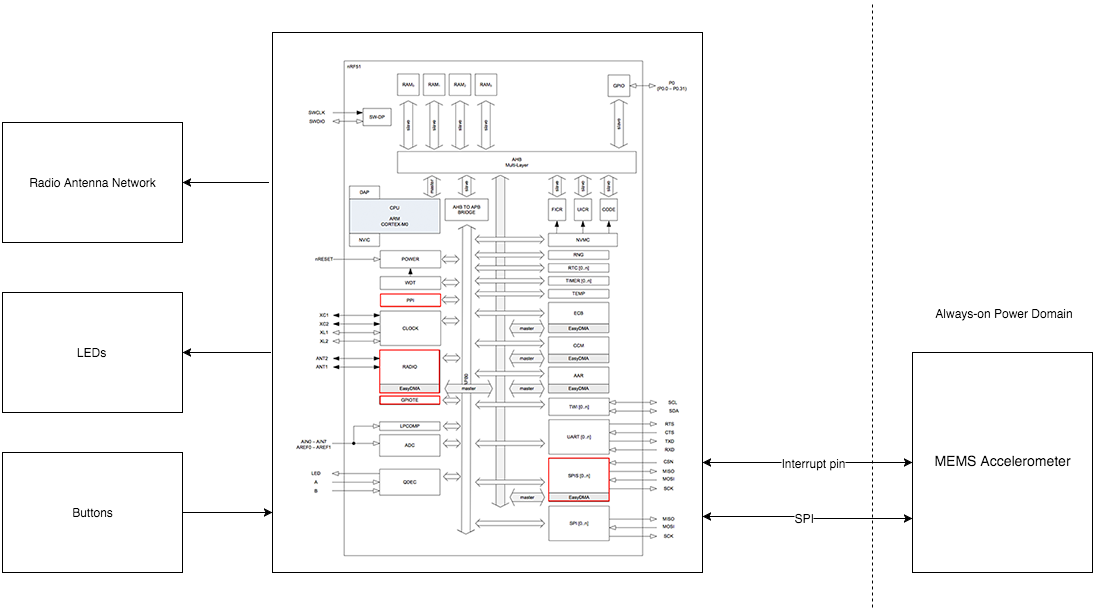
\includegraphics[scale=0.44]{fig/sys_arch.png}
\caption{Reference Board Architecture. nRF51 block diagram from \cite{nrf51}}
\label{fig:nrf51}
\end{figure}